\section{Materials and methods}

In this section we introduce the empirical data, the experiment protocol and the simulation model we use in the experiment. 

\subsection{Empirical data}

We examine data from three real-world online communities. All three use the same software (Drupal 7), are roughly comparable in size and are used by practitioners and interested citizens to publicly discuss issues that have a collective dimension. They are modelled as interaction networks, in which nodes are registered users and edges represent comments. The presence of an edge from Alice to Bob indicates that Alice has commented content authored by Bob at least once. The resulting graphs are directed ("Alice comments Bob'' is not equivalent to "Bob comments Alice'') and weighted (Alice can write multiple comments to Bob's content; the edge's weight is equal to the number of comments written). Table \ref{table:empiricalData} presents some descriptive statistics about them. 

\begin{itemize}
\item \emph{InnovatoriPA} is a community of (mostly) Italian civil servants discussing how to introduce and foster innovation in the public sector. It does not employ any special onboarding or moderation policy.
\item \emph{Edgeryders} is a community of (mostly) European citizens, discussing public policy issues from the perspective of grassroot activism and social innovation. It adopts a policy of onboarding new members, as described in section I.
\item \emph{Matera 2019} is a community of (mostly) citizens of the Italian city of Matera and the surrounding region, discussing the city's policies as it made a bid to be appointed European Capital of Culture 2019. It adopts a policy of onboarding new members, as described in section I.
\end{itemize}


\begin{table*}[t]
\centering 
\begin{tabular}{| c | c | c | c |} 
\hline 
& Innovatori PA & Edgeryders & Matera2019\\ 
& \emph{``no special policy''} & \emph{``onboard new users''} & \emph{``onboard new users''}\\ 
\hline 
In existence since & December 2008 & October 2011 & March 2013 \\
Accounts created & 10,815 & 2,419 & 512 \\
\hline 
Active participants (nodes) & 619 & 596 & 198 \\
Number of edges (weighted) & 1,241 & 4,073 & 883 \\
\hline 
Average distance\footnote{The average distance of a network is the number of steps it takes to go from a node in the network to another, averaged across all start nodes and all destination nodes. This concept was made popular by the famous ?Six degrees of separation? experiment conducted by Stanley Milgram in the 1960s \cite{milgram1967small}.} & 3.77 & 2.34 & 2.51 \\
Maximum degree & 155 & 238 & 46 \\
Average degree & 2.033 & 6.798 & 4.454 \\
\hline 
\% nodes with $d_+(n) = 0$ & 0.657 & 0.138 & 0.227 \\
\% nodes with $d_+(n) = 1$ & 0.141 & 0.159 & 0.182 \\
\% nodes with $d_+(n) = 2$ & 0.065 & 0.125 & 0.121 \\
\% nodes with $d_+(n) > 2$ & 0.137 & 0.579 & 0.470 \\
\hline 
\end{tabular}
\caption{Comparing interaction networks three online communities}
\label{table:empiricalData}
\end{table*}

A glance at their respective visualizations (Figure \ref{fig:NetViz}) shows that the interaction networks of the three online communities have very different topologies. Innovatori PA displays more obviously visible hubs than the other two. 

\begin{figure}
\centering
	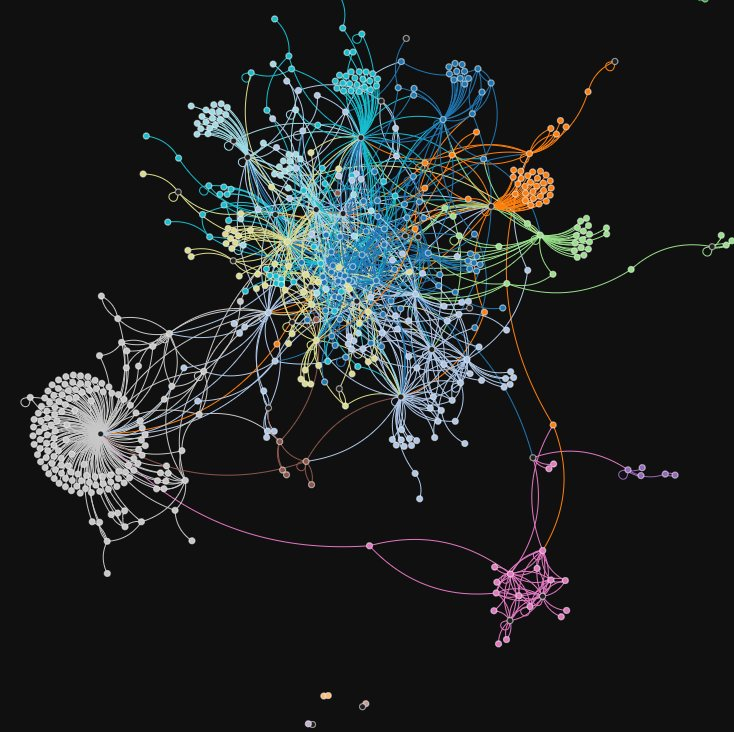
\includegraphics[width=.9\linewidth]{innovatoripa_01.jpg}\label{fig:InnoNet}
	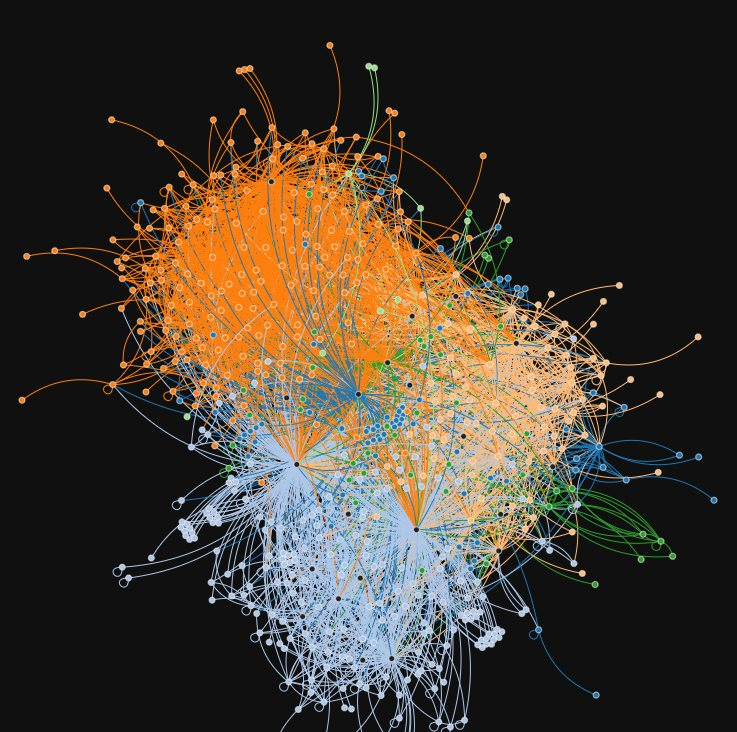
\includegraphics[width=.9\linewidth]{edgeryders_02.jpg}\label{fig:EdgeNet}
	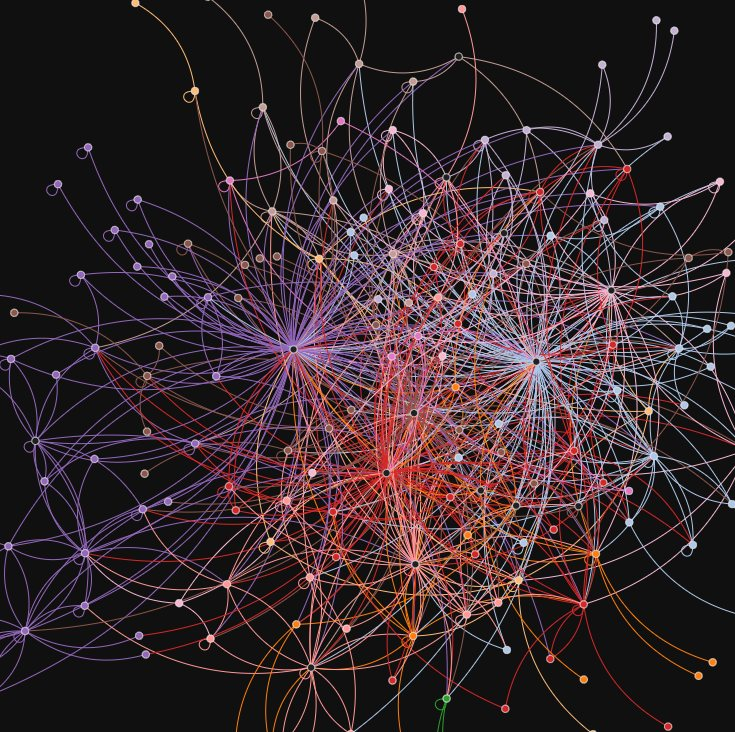
\includegraphics[width=.9\linewidth]{matera2019_01.jpg}\label{fig:MT2019Net}
  %\subfloat[][]{}
  %\subfloat[][]{}
  \caption{Interaction networks of three small online communities. Innovatori PA (top) does not have an onboarding policy in place, whereas the other two do. } 
 \label{fig:NetViz}
\end{figure}

We fit power laws in-degree distributions of these three online communities, as of early December 2014. Next, we tested the hypothesis that degree distributions follow a power law, as predicted by the theory. This was done in the following way:
\begin{enumerate}
\item first, we fitted power functions to the entire support of each in-degree distribution, i.e. for any degree greater than or equal to 1. 
\item next, we fitted power functions to the right tail of each in-degree distribution, i.e. for any degree greater than or equal to $k_{min}$, where $k_{min}$ is the in-degree that minimizes the Kolmogorov-Smirnov distance between the fitted function and the data with in-degree $k>=k_{min}$.
\item finally, we ran goodness-of-fit tests for each in-degree distribution and for fitted power functions as described in both 1 and 2. The null hypothesis tested is that the observed distribution is generated by a power function with exponent $\alpha$. We used a test based on comparing the Kolmogorov-Smirnov $D$ statistic of the observed distribution with those of a large number of synthetic datasets drawn by the fitted power function. Such comparison is summarized in a p-value, that indicates the probability of the $D$ statistic to exceed the observed value conditional to the null hypothesis being true. Observing p-values close to 1 indicate that the power function is a good fit for the data, and do not allow rejection of the null hypothesis; p-values close to zero indicate that the power function is a bad fit for the data, and lead to to reject the null hypothesis. The rejection value is set, conservatively, at 0.1.  The method we followed is borrowed from Clauset, Shalizi and Newman \cite{clauset2009power} and is described in detail in the Appendix. 
\end{enumerate}
	
We emphasize in-degree, as opposed to out-degree, for the following reason. The Barab\'asi-Albert model and many of its extensions \cite{dorogovtsev2002evolution} have been applied to undirected as well as to directed network. However, directedness is implicit in the idea of preferential attachment; new nodes "choose" who to link to. When networks are directed, it is reasonable to expect the in-degree distribution to be the one to follow a power law. This expectation has been confirmed by empirical investigation \cite{dorogovtsev2002evolution}, supporting the conjecture that some preferential attachment is present in many in online conversation networks. As new members join, many of them will reach out to someone, and it seems to make sense that they will target highly connected individuals more. 

Results are summarised in Table \ref{table:goodnessOfFit}. 

\begin{table}[b]
\centering 
\begin{tabular}{| c | c | c | c |} 
\hline 
& exponent  & $k_{min}$ & $p$-value\\ 
\hline 
Innovatori PA  $k>=1$ & 1.611 & 1 & 0.21 \\
\hline 
Innovatori PA $k>=k_{min}$  & 1.834 & 2 & 0.76 \\
\hline
Edgeryders $k>=1$ & 1.477 & 1 & 0.00 - \emph{reject} \\
\hline
Edgeryders $k>=k_{min}$ & 2.250 & 5 & 0.45 \\
\hline
Matera2019 $k>=1$ & 1.506 & 1 & 0.00 - \emph{reject} \\
\hline
Matera2019 $k>=k_{min}$ & 2.817 & 6 & 0.94 \\
\hline 
\end{tabular}
\caption{Testing for goodness-of-fit of power functions to interaction networks of degree distributions in three online communities.}
\label{table:goodnessOfFit}
\end{table}

As we consider the interval  $k>=1$, we find that the in-degree distribution of the Innovatori PA interaction network – the unmoderated one – is consistent with the expected behaviour of an evolving network with preferential attachment; we cannot reject the null hypothesis that it was generated by a power law. The same is not true of the other two online communities – both with onboarding policies – for which the null hypothesis is strongly rejected.  

When we consider only the tail of the degree distributions, i.e. degree distributions for $k>=k_{min}$, on the other hand, all three communities display a behaviour that is consistent with that of evolving networks with preferential attachment.

This set of results is consistent with the objectives of the onboarding policy. These consist of helping newcomers to overcome the initial difficulties associated with finding your way around an online community that they don't know yet. A successfully onboarded new user will generally have some extra interaction with existing community members with respect to ones that are left to themselves; all things being equal, we can expect this to lead to extra edges appearing in the interaction network, and interfering with the in-degree distribution that would appear in the absence of onboarding. This could explain the non-power law in-degree distribution of Edgeryders and Matera2019. On the other hand, it is reasonable to expect this interference to concern mostly low connectivity nodes: onboarding targets predominantly newcomers, and focuses on helping them through the first few successful interactions. Highly active (therefore highly connected) community members do not need to be onboarded. This could explain why, when we consider only the highly connected nodes in the distribution's upper tails, all three communities display similar behaviour, regardless of onboarding policies. 

\subsection{Experiment protocol}
The difference observed between the two communities with onboarding policies and the one without might be caused not by the policy itself, but by some other unobserved variable. To explore the issue further, we generate and compare computer simulations of interaction networks in online communities that are identical except for the presence and effectiveness of onboarding policies. Communities are assumed to grow over time, with new participants joining them in sequence; at each point in time, new edges appear; their probability of targeting an existing node grows linearly with that node's in-degree. Additionally, communities might have or not have onboarding policies. For those communities that do have them, they are modelled by means of two scalar parameters $\nu_1$  and $\nu_2$ , that vary between 0 and 1. The first one captures onboarding effectiveness;  the second one captures community responsiveness. As they get closer to 1, the community manager's onboarding action gets closer to having the desired effects. In the next subsection, we specify the model and define more specifically the meaning of both parameters.

We proceed as follows.

First, we simulate the evolution of the interaction network of a large number of online communities. Divide them into a control group (no onboarding policy) and a treatment group (presence of onboarding policy). Specifically, we simulate the evolution of the interaction network of:

\begin{itemize}
\item 100 communities with no onboarding policy. These will constitute the control group of our simulated communities. 
\item 100 communities for each couple of values of $\nu_1$  and $\nu_2$, with $\nu_1, \nu_2 = [0.2, 0.4, 0.6, 0.8, 1.0]$. These will constitute our treatment groups.
\item For each of these networks, we compute the in-degree distribution.
\end{itemize}

Next, we define the following hypotheses. 

\begin{itemize}
\item Let $C$ be the network of interaction in an online community. Denote the in-degree of nodes in the network by $k$. Let $P$ be the best-fit power-law model for the in-degree distribution of $C$.
\item \emph{Hypothesis 1}. The in-degree distribution of $C$ is generated by $P$ for any $k>=1$.
\item \emph{Hypothesis 2}. The in-degree distribution of $C$ is generated by $P$ for any $k>=k_{min}$, where $k_{min}$ is the in-degree that minimizes the Kolmogorov-Smirnov distance between the fitted function and the data over $k>=k_{min}$.
\end{itemize}

Finally, we test Hypothesis 1 and 2 on each of the 3800 in-degree distributions generated. We do this using the goodness-of-fit tests proposed by Clauset et.al. \cite{clauset2009power} and illustrated in detail in the Appendix.
We expect to obtain the following:

\begin{itemize}
\item In the control group, both Hypothesis 1 and Hypothesis 2 are true. 
\item In the treatment group with fully effective onboarding Hypothesis 1 is false and Hypothesis 2 is true. 
\item In the intermediate situations of partially ineffective onboarding, Hypothesis 1 can be true or false, according to the value of formula. Hypothesis 2 is true.
\end{itemize}


\subsection{The simulation model}

Our computer model simulates the growth of an interaction network in an online community with and without onboarding.  

\subsubsection*{Without onboarding}

We use the model without onboarding to generate the networks in our control group. Its growth mechanism for the network to grow is based on preferential attachment, consistently with the Barab�si-Albert tradition. We follow the more general formulation of Dorogovtsev and Mendes \cite{dorogovtsev2002evolution}.
\begin{itemize}
\item A network is initialized, consisting of two reciprocally connected nodes
\item At each time step, one new node ��\textendash   representing a participant in the online community \textendash �� appears in the network. 
\item At each time step, $m$ new edges \textendash   representing comments \textendash   appear in the network. The source of each edge is drawn at random from the uniform distribution of the existing nodes\footnote{This represents a departure from \cite{dorogovtsev2002evolution}, where edge sources are assumed to be unspecified. We need to specify edge sources in order to conform to the data model of the network analysis softwares we are using; this, however, does not have any analytical implications, as both \cite{dorogovtsev2002evolution} and we focus on the in-degree distribution.}. Its target is chosen according to the following rule: the probability that the new edge points to node $s$ is proportional to $k(s) + A$ where $A$ is a parameter representing additional attractiveness of the node.
\end{itemize}

\subsubsection*{With onboarding}

We use a variant of the above model that includes onboarding to generate the networks in our treatment group. The variant consists simply of the model without onboarding, to which further steps are added as follows.
\begin{itemize}
\item At each timestep, one edge is directed towards the newcomer node. This is meant to represent the community manager's onboarding action described in section 1. 
\item At each timestep, with probability $\nu_1$, one edge is added. Its source is the newcomer node; its target is chosen according to the following rule: the probability that the new edge points to node $s$ is proportional to $k(s) + A$ where $A$ is a parameter representing additional attractiveness of the node. This is meant to represent the newcomer's reaction to the community manager's onboarding activity; as a result of the latter, the newcomer becomes active and reaches out to someone in the community, as advised by the community manager. We assume that community managers will normally incline to point newcomers to existing users who are reputed to be interesting conversationalists, and that the characteristic of being interesting conversationalists is correlated with node in-degree. $\nu_1$ can be thought of as representing \emph{onboarding effectiveness}. More skilled community managers will be more persuasive in inducing newcomers to reach out and engage in the conversation taking place in the online community.
\item At each timestep, with probability $\nu_2$, one edge is added. Its source is drawn at random from the uniform distribution of the existing nodes; its target is the newcomer node. This represents a successful onboarding outcome: the new participant, by becoming active, has attracted the attention of some existing participant, who has engaged with her. The new participant, no longer isolated, is now in conversation. $\nu_2$ can be thought of as representing \emph{community responsiveness}. As it increases, the efforts of newcomers to engage in conversation become more likely to be reciprocated.
\end{itemize}
